
\begin{definition}{7.2.338}\label{def:7-2-338}
令
\begin{equation}
\begin{aligned}
\widehat{\mathfrak C}_X(L'_1)
={}&C_b([0,1]^2\times L'_1,(\lambda_0,\lambda'_1))\\
&\vee_r C_X([0,1]^2\times L'_1,(\lambda_0,\lambda'_1))\\
&\vee_r C_c([0,1]^2\times L'_1,(\lambda_0,\lambda'_1)).
\end{aligned}
\tag{7.2.339.1}\label{eq:7-2-339-1}
\end{equation}
（参见图式~\ref{diag:7-2-21}、
引理~\ref{lem:7-2-285}
及图式~\ref{diag:7-2-26}。）
记 $C_0=C(L'_1,\lambda'_1)$。
再定义
\begin{equation}
\begin{aligned}
\mathfrak C_X^{s=s_0}(L'_1)
={}&C_b^{s=s_0}
([0,1]_r\times L'_1,(\lambda_0,\lambda'_1))\\
&\vee_r C_X^{s=s_0}
([0,1]_r\times L'_1,(\lambda_0,\lambda'_1))\\
&\vee_r C_c^{s=s_0}
([0,1]_r\times L'_1,(\lambda_0,\lambda'_1)).
\end{aligned}
\tag{7.2.339.2}\label{eq:7-2-339-2}
\end{equation}
并定义如下两映射：
\[
\begin{aligned}
\mathfrak H_X\colon\;&
C(L_0,\lambda_0)
\longrightarrow\widehat{\mathfrak C}_X(L'_1),\\
\mathcal F_X^{s=s_0}\colon\;&
C(L_0,\lambda_0)
\longrightarrow\mathfrak C_X^{s=s_0}(L'_1).
\end{aligned}
\]
\begin{equation}
\mathfrak H_X
=\mathfrak H_b\vee_r
\mathfrak f^{\{\Phi_{r,s}\}_{r,s}}
\vee_r\mathfrak H_c,
\tag{7.2.340.1}\label{eq:7-2-340-1}
\end{equation}
\begin{equation}
\mathcal F_X^{s=s_0}
=\mathcal F_b^{s=s_0}
\vee_r\mathfrak f^{\{\Phi_{r,s_0}\}_r}
\vee_r\mathcal F_c^{s=s_0}.
\tag{7.2.340.2}\label{eq:7-2-340-2}
\end{equation}
还可定义如下评价映射：
\[
\operatorname{Eval}_{s=s_0}\colon
\widehat{\mathfrak C}_X(L'_1)
\longrightarrow
\mathfrak C_X^{s=s_0}(L'_1),
\]
它满足
\begin{equation}
\operatorname{Eval}_{s=s_0}\circ\mathfrak H_X
=\mathcal F_X^{s=s_0}.
\tag{7.2.341}\label{eq:7-2-341}
\end{equation}
\end{definition}

下列图式~\ref{diag:7-2-27} 交换：

\par\medskip\noindent\begin{minipage}{\textwidth}
\centering
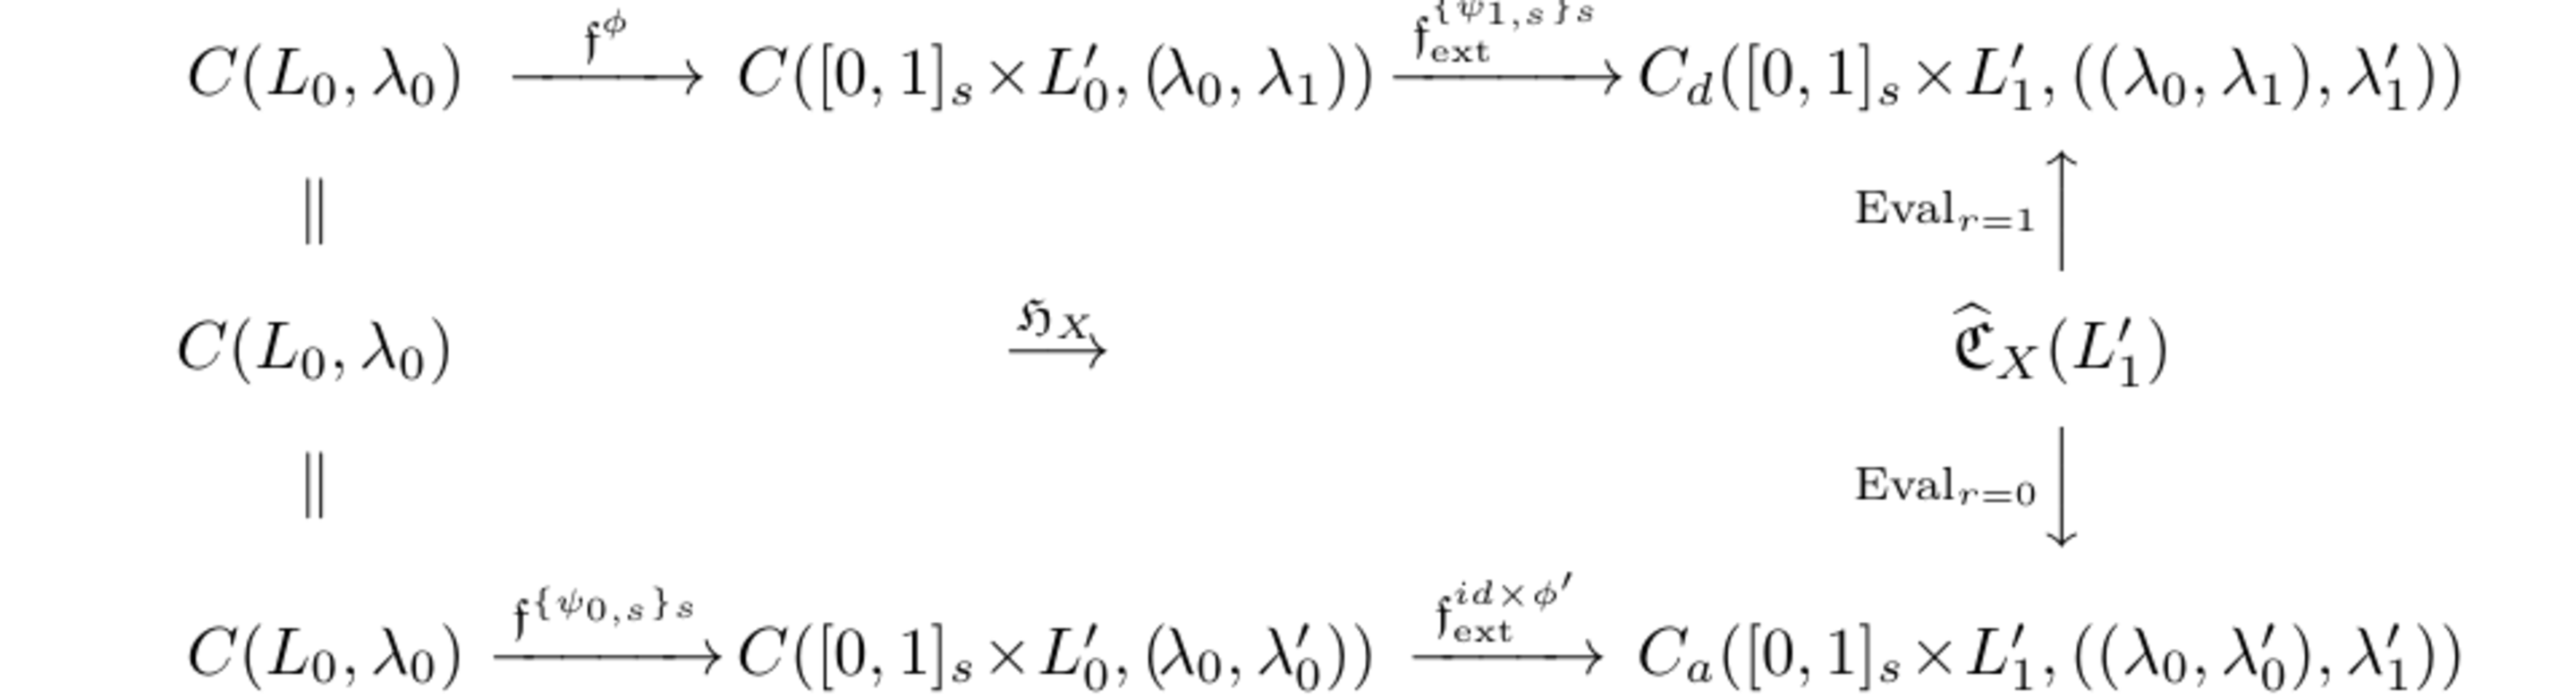
\includegraphics[width=\textwidth]{chapters/ch07-transversality/figures/phys-571-diagram-7-2-27-math-final-crop.png}
\par{\renewcommand{\thefigure}{7.2.27}\refstepcounter{figure}
\normalfont\bfseries 图式~\thefigure\label{diag:7-2-27}}
\end{minipage}\par\medskip
图式~\ref{diag:7-2-27}
的标注保留原样\translatornote{原书上行中点写
$C([0,1]_s\times L'_0,(\lambda_0,\lambda_1))$；
但入射的 $\mathfrak f^\phi$ 的靶
及图式 7.2.25 的相应顶点均在 $L_1$ 上。
此处预期底空间为 $L_1$，
故保留源图并提示这一型别不合。}。
